% FILIPPO
% 2. PLP. The customer can:
%     a. Select multiple product items;
%     b. Add the selected products to the shopping cart;
%     c. Navigate to the shopping cart page;

\UC{Ordinamento prodotti PLP}

\begin{figure}[H]
	\centering
	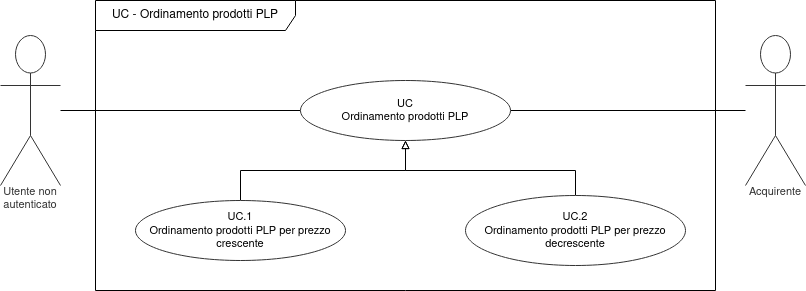
\includegraphics[width=\textwidth]{Immagini/DiagrammiUC/OrdinamentoProdotti.png}
	\caption{Diagramma di \actualUC: Ordinamento prodotti PLP} 
	\label{fig:OrdinamentoProdotti}
\end{figure}

L'utente non autenticato o l'acquirente può ordinare i prodotti risultanti dalla ricerca effettuata in precedenza.
\begin{itemize}
	\item \textbf{Attori Primari:} Acquirente; Utente non autenticato.
	\item \textbf{Precondizione:} L'attore è nella PLP e ha selezionato l'ordinamento.
	\item \textbf{Postcondizione:} I prodotti nella pagina vengono ordinati secondo l'ordinamento selezionato.
	\item \textbf{Scenario Principale:} L'attore può ordinare i prodotti nella PLP scegliendo tra i seguenti ordinamenti
	\begin{itemize}
		\item Ordinamento crescente \actualUC.1
		\item Ordinamento decrescente \actualUC.2
	\end{itemize}
	\item \textbf{Scenario Alternativo:} Se la ricerca effettuata non ha prodotto alcun risultato, l'attore non potrà selezionare nessun tipo di ordinamento.
\end{itemize}
\resetSubUC

\subUC{Ordinamento prodotti PLP per prezzo crescente}
L'utente non autenticato o l'acquirente può ordinare i prodotti risultanti dalla ricerca effettuata in precedenza per prezzo crescente.
\begin{itemize}
    \item \textbf{Attori Primari:} Acquirente; Utente non autenticato.
    \item \textbf{Precondizione:} L'attore è nella PLP e ha selezionato l'ordinamento per prezzo crescente.
    \item \textbf{Postcondizione:} I prodotti nella pagina vengono ordinati in ordine di prezzo crescente.
    \item \textbf{Scenario Principale:} L'attore vuole ordinare i prodotti nella pagina così da averli elencati dal più economico al più costoso.
\end{itemize}

\subUC{Ordinamento prodotti PLP per prezzo decrescente}
L'utente non autenticato o l'acquirente può ordinare i prodotti risultanti dalla ricerca effettuata in precedenza per prezzo decrescente.
\begin{itemize}
    \item \textbf{Attori Primari:} Acquirente; Utente non autenticato.
    \item \textbf{Precondizione:} L'attore è nella PLP e ha selezionato l'ordinamento per prezzo decrescente.
    \item \textbf{Postcondizione:} I prodotti nella pagina vengono ordinati in ordine di prezzo decrescente.
    \item \textbf{Scenario Principale:} L'attore vuole ordinare i prodotti nella pagina così da averli elencati dal più costoso al più economico.
\end{itemize}

\UC{Aggiunta al carrello dalla PLP}
L'utente non autenticato o l'acquirente può aggiungere al carrello i prodotti direttamente dalla PLP, senza che debba per forza entrare nella \glo{PDP} specifica del prodotto.
\begin{itemize}
    \item \textbf{Attori primari:} acquirente o  utente non autenticato.
    \item \textbf{Precondizione:} l'attore è nella PLP;
    \item \textbf{Postcondizione:} l'attore rimane nella PLP e al carrello è stato aggiunto il prodotto nella quantità desiderata;
    \item \textbf{Scenario principale:} L'attore vuole comprare più quantità di un prodotto e in tal caso:
    \begin{itemize}
        \item Preme sull'azione di aggiunta al carrello del prodotto scelto tra i prodotti visualizzati;
          \item (UC) - Modifica la quantità di prodotto da inserire nel carrello;
        \item Conferma la volontà di aggiungere il prodotto nel carrello con la quantità impostata.
    \end{itemize}
\end{itemize}
